\chapter{Charge-oscillation nature of $\uppi$--$\uppi$ interactions}\label{chap:pi-pi}

{\sffamily\mathversion{sans} This chapter uses the decomposition of the coupled-oscillator wave function and the expression for the coupled-oscillator density from Chapter~\ref{chap:mbd} to give a clear physical picture of binding in $\uppi$--$\uppi$ stacked systems.
This study illustrates the benefits of formulating a method (MBD in this case) via a model Hamiltonian, which gives automatically access not only to the energy but also to the wave function.
The results show that the $\uppi$--$\uppi$ stacking is associated with vdW interactions originating from collective nonlocal oscillations, which explains the difficulties of pairwise vdW methods to describe these systems accurately.
It is demonstrated that besides interaction energies, the harmonic oscillators can yield also a good prediction of the vdW-associated redistribution of the electron density, which then partially motivates the focus on the spatial distribution of the local polarizability in Chapter~\ref{chap:polarizability}.
Most of the results in this chapter have been published in \citep{HermannNC17}.
The diffusion quantum Monte-Carlo calculations were done by prof.\ Dario Alfè from University College London.
}

\section{Background}

Noncovalent $\uppi$--$\uppi$ interactions is the name given by chemists to the common stacking pattern of planar or locally planar molecular systems that are characterized by $\uppi$ orbitals---the aromatic systems.
The binding pattern having its own name is supported by its importance in chemistry and biology.
$\uppi$--$\uppi$ interactions play a key role in the formation of the double-helix structure of RNA and DNA by stabilizing the stacked nuclobases \citep{HunterJMB93}.
In general, they contribute to most chemical and biological self-assembly mechanisms, including protein folding \citep{ArigaSTAM08,ZhangNB03}.
Biochemical recognition, inherent in drug design, is often driven by stacking of aromatic compounds \citep{MeyerACIE03}.
The recently established field of vdW heterostructures studies layered materials with functional properties designed by precise ordering of layers \citep{GeimN13}.
The stability of such structures is largely driven by aromatic stacking interactions.

Despite their distinct nature, $\uppi$--$\uppi$ interactions are just a result of the fundamental long-range electron interactions, and as such can be calculated with excellent precision using high-level methods of quantum chemistry, when the systems are small enough that such calculations are feasible.
Benzene dimer, a prototypical aromatic stacked system, has been investigated by many authors using methods such as the coupled-cluster theory and symmetry-adapted perturbation theory (SAPT) \citep{HobzaJPC96,KimCR00,SinnokrotJACS02,SinnokrotJPCA06,DiStasioCPL07,PodeszwaJPCA06}, and these studies determined its binding energy of $\sim$2.7\,kcal/mol to within 2\% accuracy.
But due to their complex formulations, these methods cannot provide any understanding of the binding energy, and hence the stacking pattern, in terms of the underlying electronic motions.
The SAPT provides decomposition of the total binding energy in terms of exchange, electrostatic, induction, and dispersion components, but these decompositions are not in any way qualitatively specific to $\uppi$--$\uppi$ interactions.
Earlier, \citet{HunterJACS90} tried to give a qualitative picture of $\uppi$--$\uppi$ interactions in terms of the characteristic arrangement of permanent quadrupole moments in aromatic systems, but this model is not supported by the high-level calculations.
This led some to suggest that there is indeed nothing electronically special about $\uppi$--$\uppi$ stacking and that the use of the term $\uppi$--$\uppi$ ``interactions'' cannot be justified.

On the other hand, long-range plasmon oscillations in low-dimensional zero-gap materials, including the aromatic graphene, lead to characteristic power laws in the dependence of the binding energy on distance~\cite{DobsonPRL06,BordagPRB06}.
The zero electronic gap in graphene is directly related to the system of conjugated $\uppi$ bonds, and so at least in this particular case, $\uppi$--$\uppi$ interactions are supported by a particular collective electronic motion.
This view was further supported by~\citet{MisquittaPRB10}, who showed that the smallness of the gap is inversely proportional to the length scale of the plasmon oscillations and hence the electronic response.
In contrast to the high-level methods of quantum chemistry, these plasmon-based models give a good qualitative understanding of the interactions, but cannot provide quantitative description of the binding.
This is caused by the analytic formulation of the models, which enables deriving the qualitative results, but cannot be easily extended to the microscopic atomic description.

The MBD method, combined with semilocal KS-DFT calculations, reaches close to the quantitative accuracy of high-level electronic-structure methods, while giving the qualitative insight of simple response models.
Furthermore, it is easily applicable to large systems, which are inaccessible to the methods of quantum chemistry.
The ability to provide insight stems from the formulation of the MBD method as a simple Hamiltonian model.
This gives access to not only the energy, but also the underlying wave function.
Using the tools presented in Chapter~\ref{chap:mbd}, this wave function can be analyzed, and this analysis can provide answers to the question whether the $\uppi$--$\uppi$ stacking is characterized by some specific electronic phenomenon.

\section{Benchmarking MBD binding energies with DQMC}

\begin{figure}
\makebox[\textwidth][c]{
\begin{tikzpicture}
\node[below right, anchor=base] at (0,0) {{\bfseries a}};
\node[below right] at (-.5,.5) {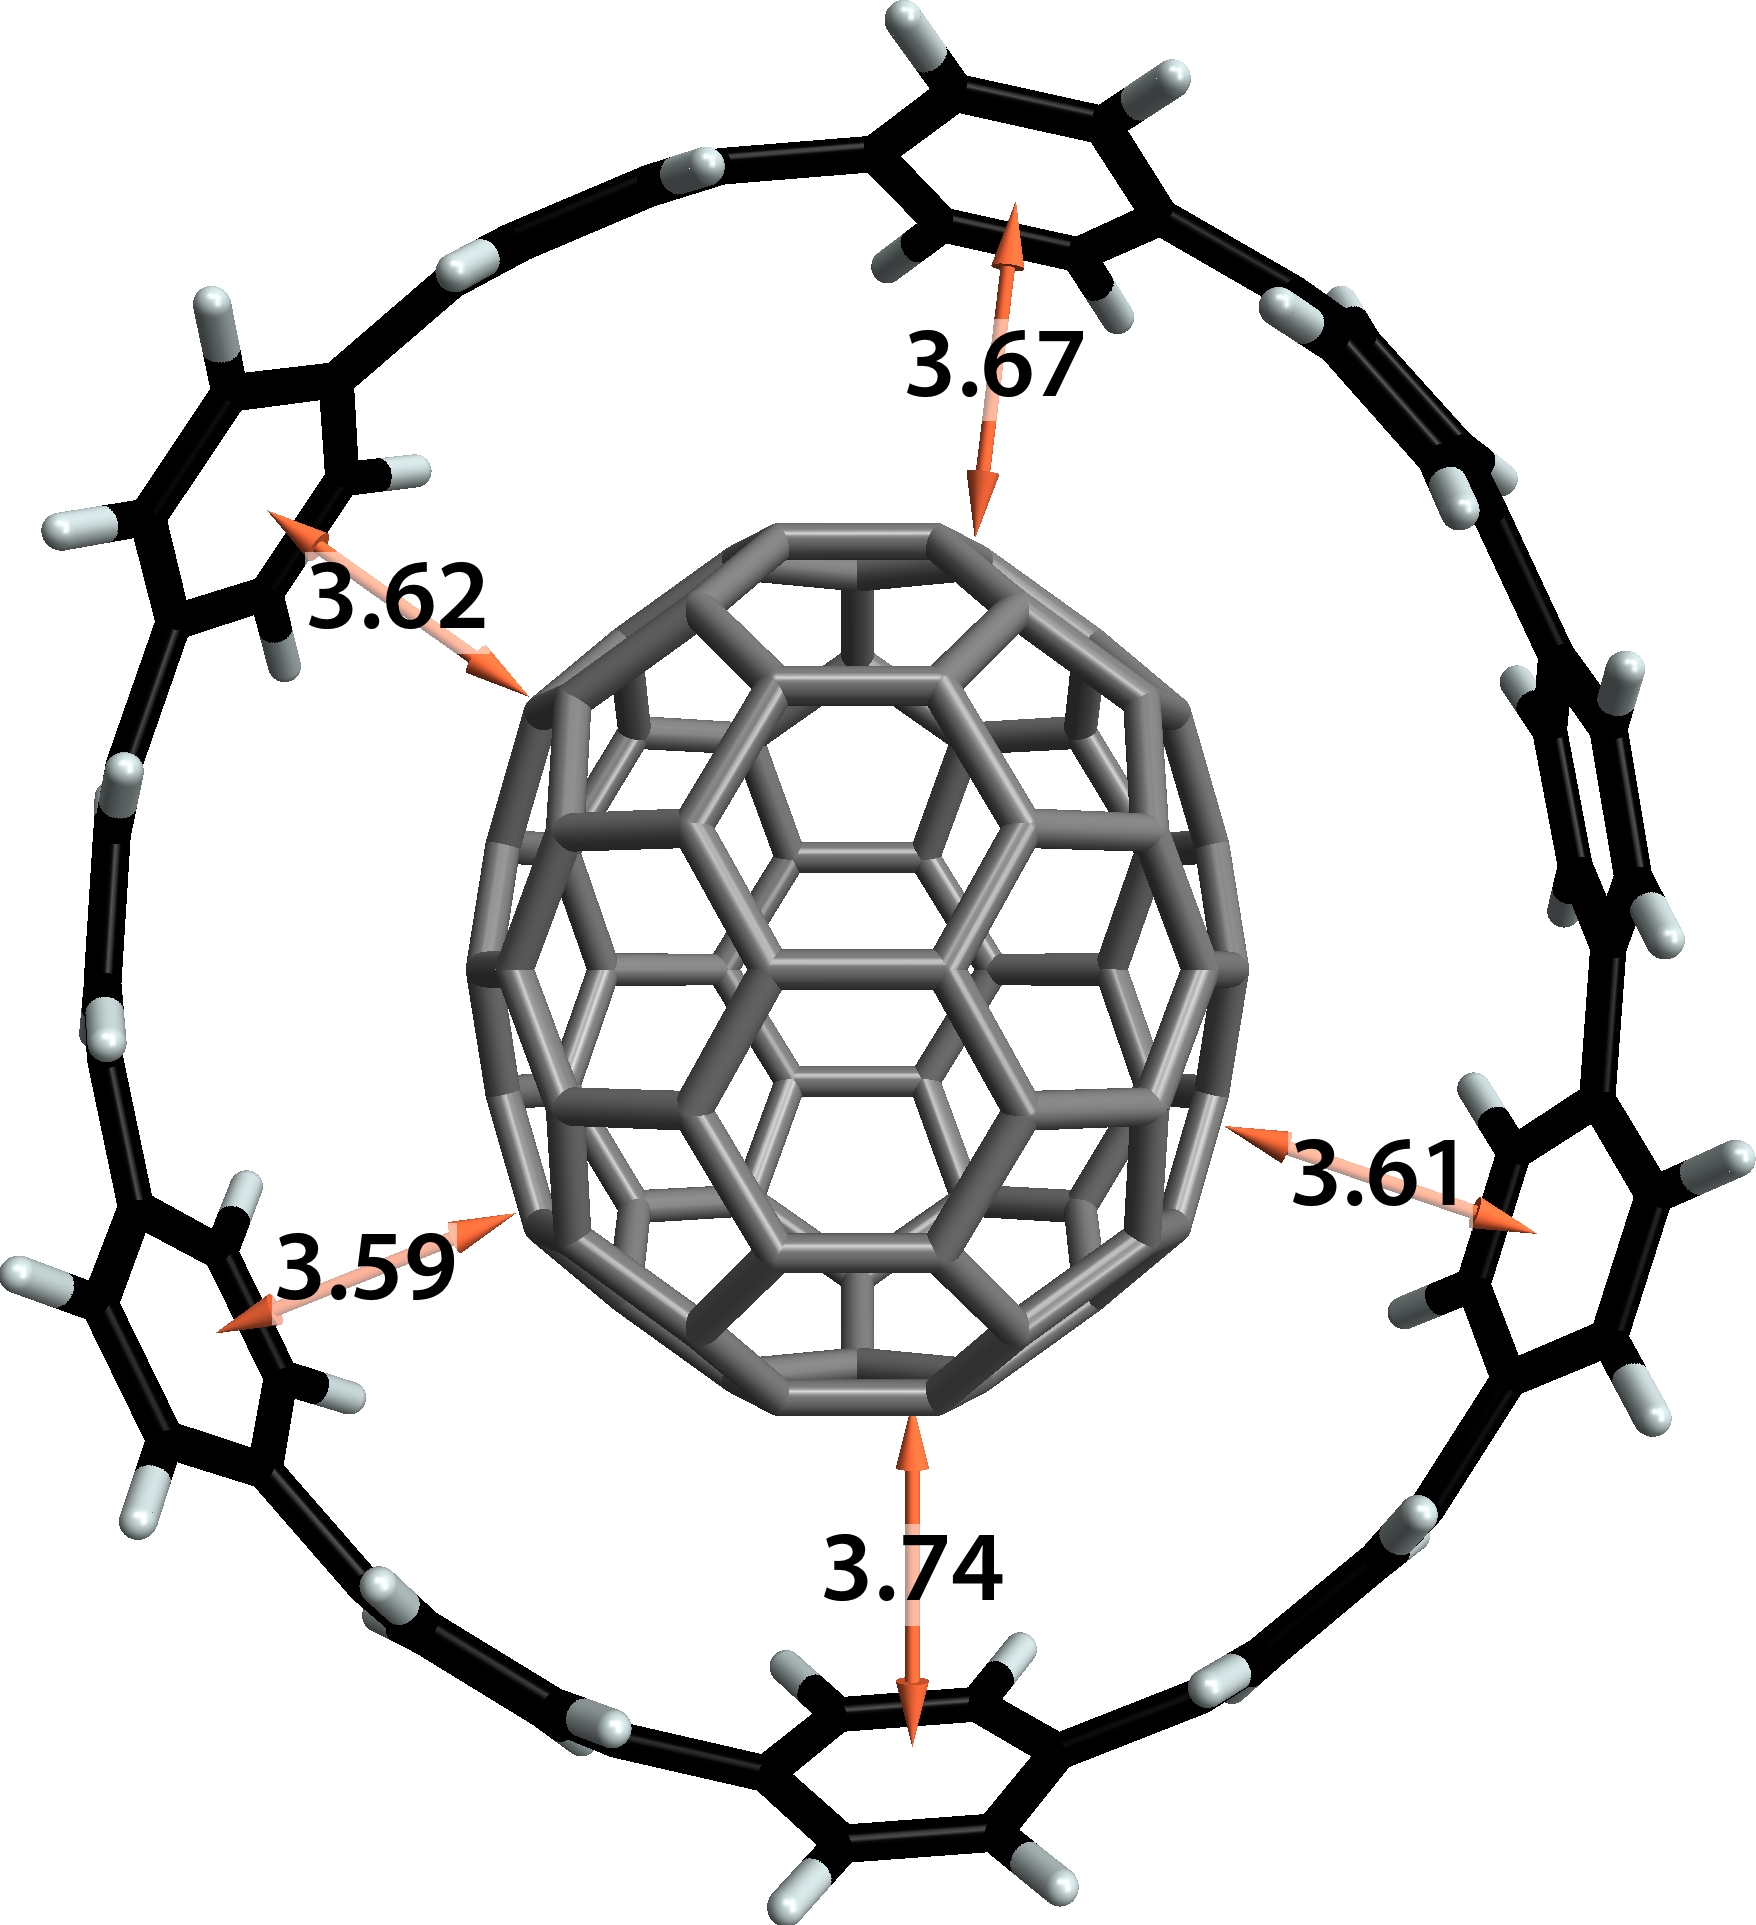
\includegraphics[width=\linewidth/3]{media/geom-cpp-11.png}};
\node[below right, anchor=base] at (\linewidth/3-5,0) {{\bfseries b}};
\node[below right] at (\linewidth/3-6,.5) {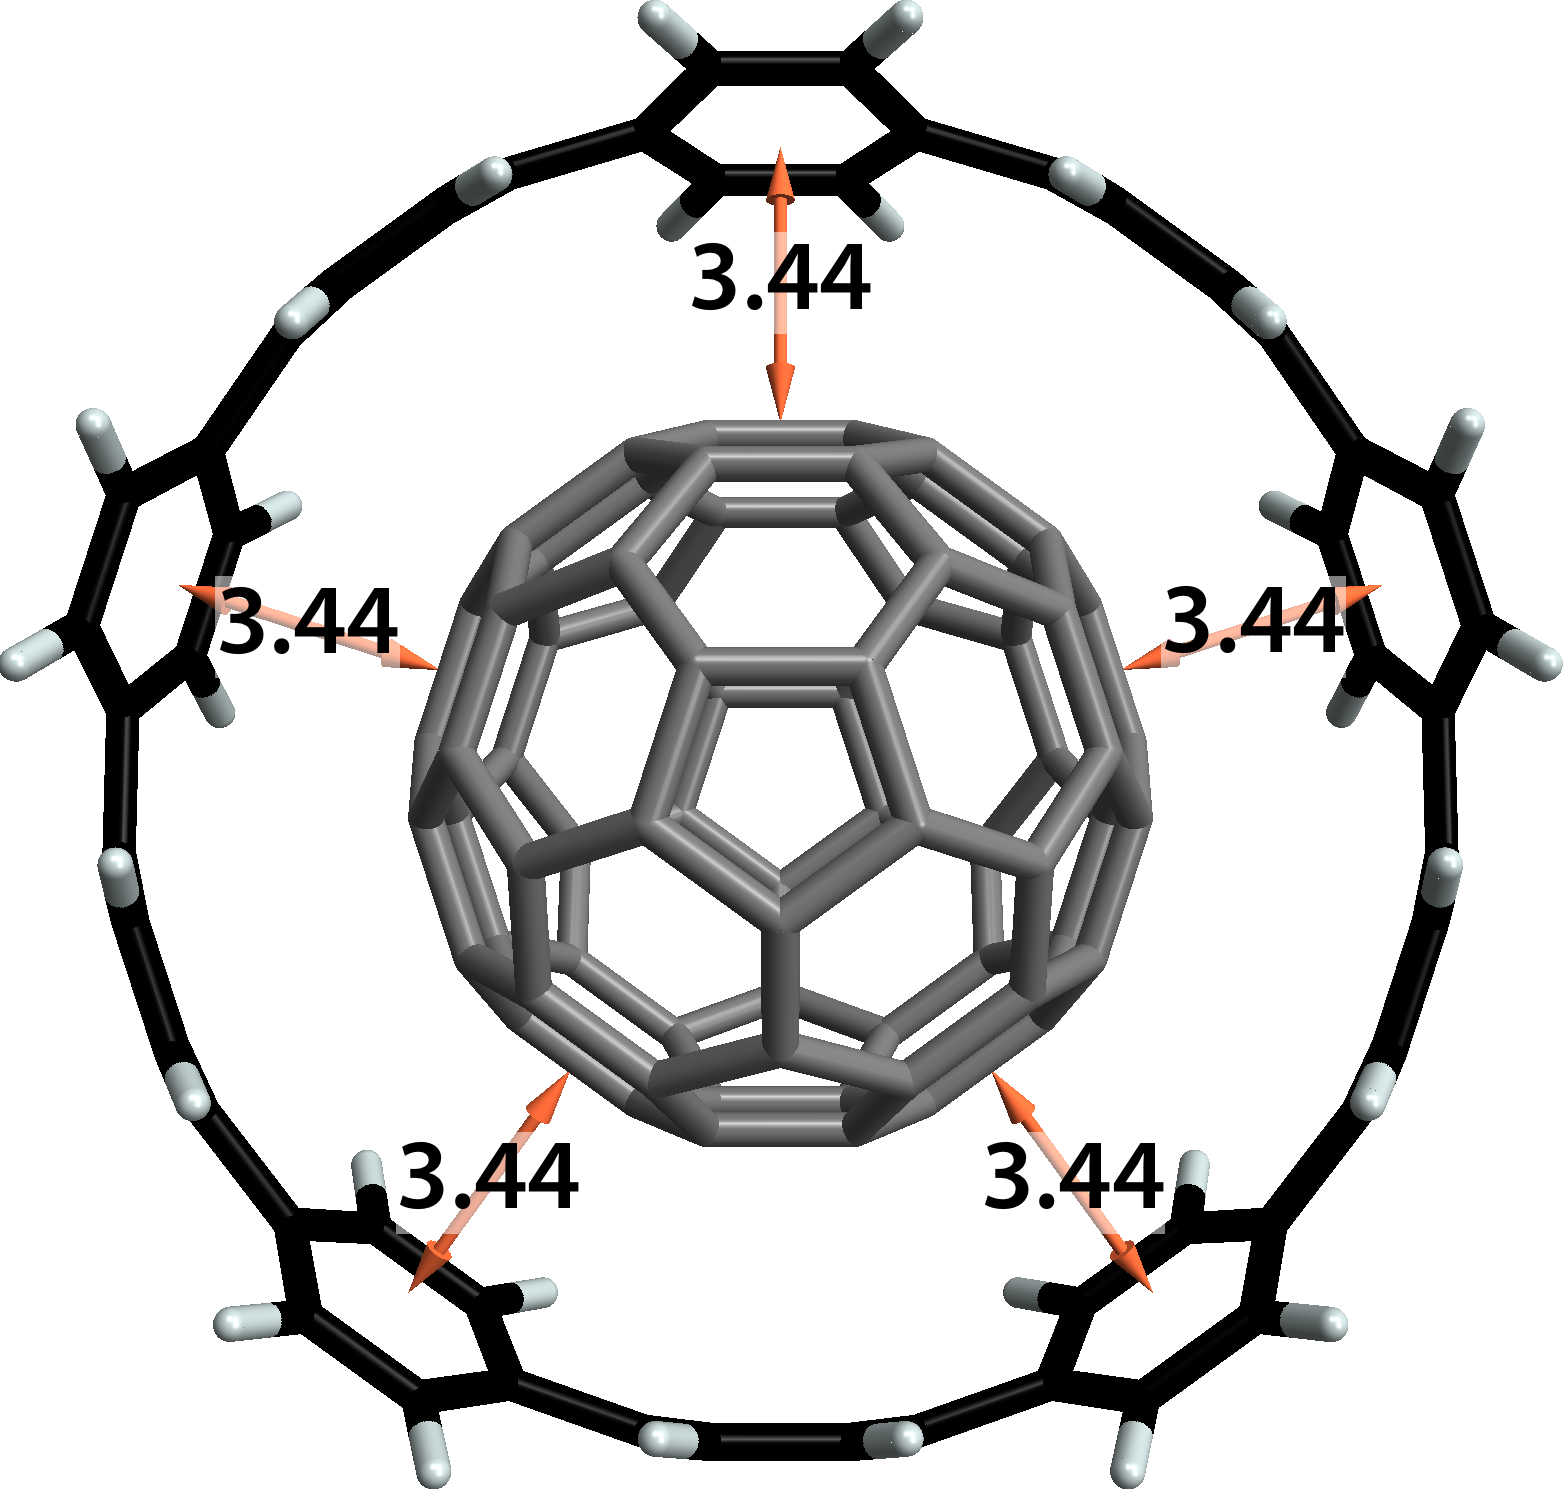
\includegraphics[width=\linewidth/3]{media/geom-cpp-10.png}};
\node[below right, anchor=base] at (2*\linewidth/3,0) {{\bfseries c}};
\node[below right] at (2*\linewidth/3-.5,.5) {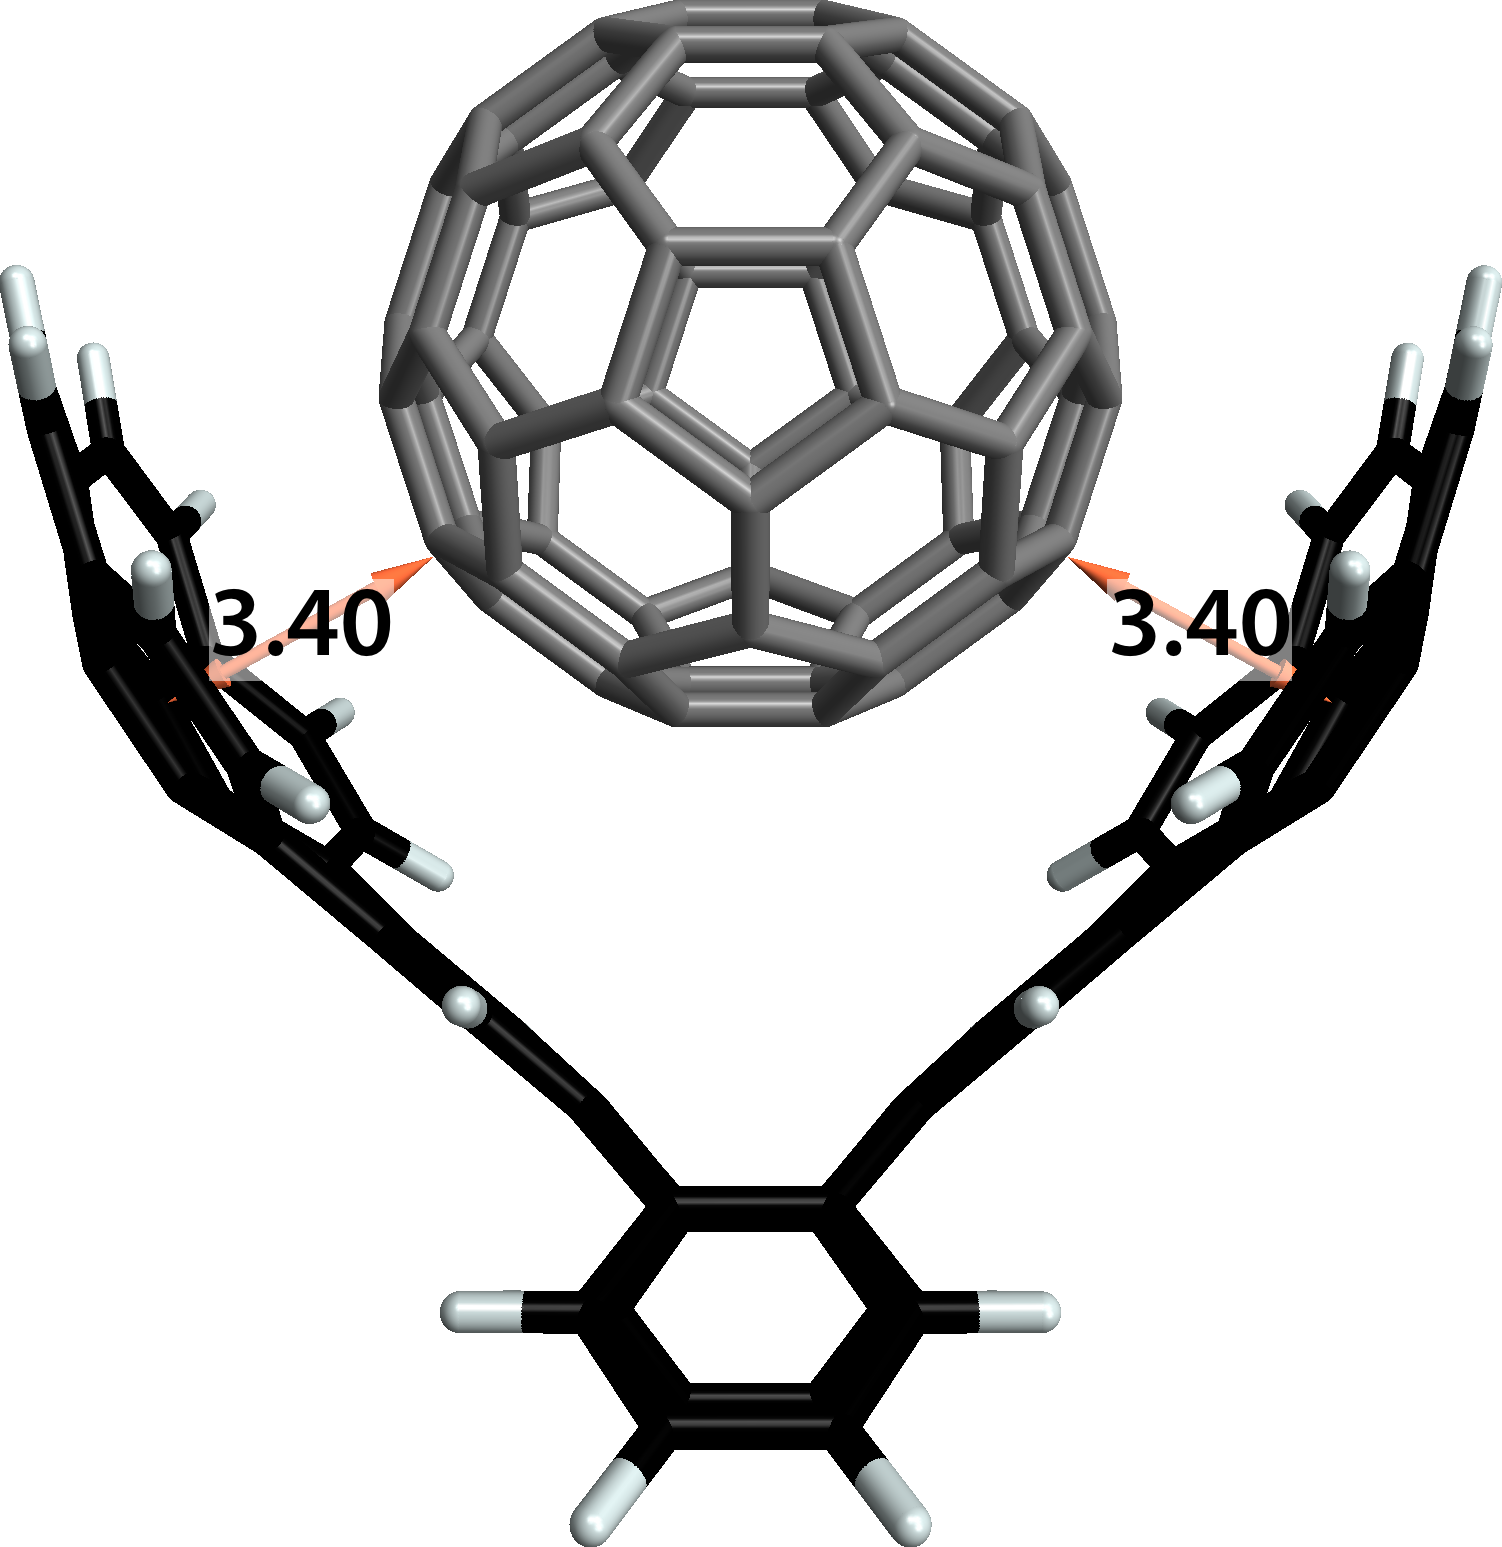
\includegraphics[width=\linewidth/3]{media/geom-catcher.png}};
\end{tikzpicture}
}
\caption{\textbf{Equilibrium structures of supramolecular complexes of fullerene C$_{70}$.}
The arrows denote the distances from centers of 6-member aromatic rings to the nearest point on the fullerene.
The three host molecules are [11]-cycloparaphenylene (\textbf a), [10]-cycloparaphenylene (\textbf b), and the ``buckycatcher'' C$_{60}$H$_{24}$ (\textbf c) \citep{SygulaJACS07}.
}\label{fig:pipi-structures}
\end{figure}

In general, any interpretations of the results by any DFT+vdW approach are complicated by the ambiguity in the range separation between the short-range DFT part and long-range vdW part.
To avoid this issue, we studied $\uppi$--$\uppi$ stacking pattern in supramolecular complexes, where the binding energy is dominated by the long-range part, and all qualitative answers are therefore delegated to the analysis of the MBD method.
Furthermore, supramolecular chemistry is a relatively new field with much focus on the design of novel complexes with targeted properties~\cite{KawaseSCoFaCN12}.
As such, a good intuitive understanding of the involved interactions is especially important.

We chose three supramolecular complexes (Figure~\ref{fig:pipi-structures}) as representative examples of $\uppi$--$\uppi$ interactions, which will be denoted $C_1$, $C_2$, and $C_3$ in the order introduced below.
All three are already synthesized host--guest systems, in which the guest molecule is the C$_{70}$ fullerene with $D_{5\mathrm h}$ symmetry, sometimes also called ``rugbyballene'' for its elongated shape.
Two host molecules are [11]- and [10]-cycloparaphenylenes (CPP) \citep{JastiJACS08}, which are the simplest precursors of $(11,11)$ and $(10,10)$ armchair nanotubes, and the whole complexes with the fullerene molecule are therefore precursors of ``nanotube pea pods'' \citep{OkadaPRL01,MonthiouxC02}.
The third host is the C$_{60}$H$_{24}$ tweezers-like molecule that was specifically designed as a host for the C$_{60}$ fullerene \citep{SygulaJACS07}, hence the name ``buckycatcher''.
The buckycatcher--fullerene complex is a typical example of convex--concave systems, which are investigated as potential ball-and-socket joint interfaces \citep{KawaseCR06,KawaseSCoFaCN12}.
All three complexes were previously investigated theoretically using the DFT+D3 approach \citep{GrimmeCEJ12,RisthausJCTC13,AntonyCC15}.

Before analyzing the binding mechanism within the MBD model, we first want to verify that it describes correctly the binding energetics.
In principle, the experimental Gibbs energies of formation could serve as reference data against which the calculated binding energies could be compared.
They were measured for all three complexes in a solution, and the obtained values are 7, 7~\cite{IwamotoCEJ13} and 5 kcal/mol~\cite{Muck-LichtenfeldPCCP10} for $C_1$ to $C_3$, respectively.
But calculation of Gibbs energies of formation in a solution from binding energies in vacuum requires further calculations of the temperature and solvation effects.
Whereas the temperature effects can be estimated relatively accurately from molecular vibrations using harmonic approximation, the quantitative uncertainty of available solvation models is substantially worse than the accuracy of state-of-the-art DFT+vdW models~\cite{YangNC13}.

To avoid these issues, we compare the DFT+MBD binding energies against a higher-level theoretical reference.
The size of the complexes prevents the use of the standard reference method of quantum chemistry, the coupled-cluster method with single, double and perturbative triple excitations (CCSD(T)).
As a feasible alternative, we chose the DQMC method (Section~\ref{sec:dqmc}), which scales much better with system size and is easily paralellizable, so that calculations on the present systems are feasible.
The only potential systematic error in the DQMC method, caused by the fixed-node approximation, has been shown to be negligible for binding energies of vdW complexes~\cite{DubeckyJCTC13}, yielding results within 0.1\,kcal/mol of the CCSD(T) method.

\begin{figure}
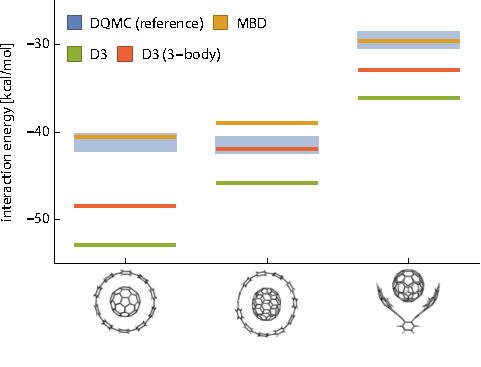
\includegraphics[width=4in]{media/master-table.pdf}
\caption{\textbf{Binding energies of supramolecular complexes with different methods.}
The blue box for the DQMC method has a height of 2\,kcal/mol and denotes the statistical uncertainty (70\%) of the result.
}\label{fig:pipi-energies}
\end{figure}

The binding energies of the three complexes calculated with the DQMC, DFT+MBD and DFT+D3 methods are compared in Figure~\ref{fig:mbd-convergence}.
The energies of the complexes were calculated with respect to the energies of the relaxed components.
The equilibrium geometries as well as the DFT+D3 results were taken from refs.\ \cite{RisthausJCTC13} ands \citep{AntonyCC15}.
We used the GGA functional of \citet*{PerdewPRL96} (PBE) as the short-range complement of the MBD method.
In Chapter~\ref{chap:xc-functionals}, we show that this functional is particularly consistent in the degree of short-range XC energy that it captures.
Being a stochastic method, the DQMC energies are always calculated with a certain statistical uncertainty that can be chosen freely by the amount of computational time invested in the calculation.
Here, we chose the uncertainty of $\pm1$\,kcal/mol, which is enough to judge the accuracy of the DFT+vdW methods.
Interestingly, the ratios of the binding energies correspond quite accurately to the ratios of the Gibbs energies of formation.
This suggests that temperature and solvation effects do not differ significantly between the three complexes.

The results demonstrate that the PBE+MBD method is able to capture both absolute and relative energetics of the complexes.
The largest deviation of PBE+MBD is 2.5\,kcal/mol in the case of complex $C_2$, while the energies of the other two complexes are estimated withing the statistical error of the DQMC method.
The near-degenerate complexes $C_1$ and $C_2$ are estimated to be only 1.5\,kcal/mol apart.
In contrast, the DFT-D3 method systematically overestimates the binding energies by 7--12\,kcal/mol, and the $C_1$ and $C_2$ complexes differ by 7\,kcal/mol.
Adding the 3-body correction in D3 improves the systematic overbinding, but the relative energetics of $C_1$ and $C_2$ is not improved.
In solution at room temperature, the difference of 7\,kcal/mol between the two complexes would result in a near nonexistence of $C_2$.

\section{Analysis of nonlocal polarizabilities}

The failure of the DFT-D3 method is much larger on the relative scale than could be anticipated from its accuracy on smaller complexes, including $\uppi$--$\uppi$ complexes such as benzene dimer.
This discrepancy serves as a further motivation for understanding the specific nature of the vdW interactions in $\uppi$--$\uppi$ stacked systems.
The two main differences between the D3 and MBD methods are in the models for the atomic dynamic polarizabilities ($C_6$ coefficients) and in the truncation of the many-body expansion of the ACFD formula (D3 is truncated at second order, third with 3-body correction, MBD is not truncated).
In both methods, the polarizability models are mostly local (geometric in D3, density-based in MBD), and any deficiency of the D3 model in this regard would manifest equally in smaller systems, which is not the case, leaving the many-body effects as potential explanation for the overbinding and missing degeneracy in the D3 description.

By evaluating the MBD screening equation in~\eqref{eq:mbd-dyson} for the whole complex, and the host and guest molecules independently, the many-body effects can be formally divided into intra- and intermolecular.
Writing the dipole operator in a block form, where the blocks correspond to the host (h) and guest (g) molecules,
\begin{equation}
  \mathbf T=\begin{pmatrix}\mathbf T_\text{hh} & \mathbf T_\text{hg} \\\mathbf T_\text{hg} & \mathbf T_\text{gg}\end{pmatrix}
\end{equation}
the fully coupled nonlocal dipole--dipole polarizability of the complex has an approximately block-diagonal form,
\begin{equation}
  \boldsymbol\alpha=\boldsymbol\alpha_\text{h}\oplus\boldsymbol\alpha_\text{g}+
  \begin{pmatrix}O(\mathbf T_\text{hg}^2) & O(\mathbf T_\text{hg}) \\O(\mathbf T_\text{hg}) & O(\mathbf T_\text{hg}^2)\end{pmatrix}
\end{equation}
Here, the nonlocal polarizabilities of the isolated host and guest molecules, $\boldsymbol\alpha_\text{h}$ and $\boldsymbol\alpha_\text{g}$, capture the intramolecular many-body effects, which are manifested in nontrivial dependence of the total polarizability on system size \citep{GobreNC13,RuzsinszkyPRL12}.
Whereas the short-range screening usually depolarizes the system under the effect of a field, the long-range intramolecular correlation enhances the polarization.
As a result, the total polarizability can be both smaller or greater than the sum of atomic polarizabilities, based on the geometry, size and overall dimensionality of the system.
For instance, the bulky geometry of most fullerenes leads to smaller total polarizabilities with respect to the polarizability of $sp^2$ carbon atoms \citep{TkatchenkoPRL12}.
In contrast, linear and planar geometries often lead to larger polarizabilities, as demonstrated for example by the increased stabilization of linear acene dimers~\cite{GrimmeACIE08,EhrlichACR13}
In the CPP--C$_{70}$ complexes studied here, the electrodynamic screening decreases the total polarizability of the fullerenes by 25\% with respect to the sum of the Hirshfeld-scaled free-atom polarizabilities, whereas the polarizability of [10]- and [11]CPP is increased by 31\% and 34\%, respectively.
This small difference cannot explain the inability of the D3 method, in which the intramolecular screening is neglected, to predict the degeneracy between the two complexes.

\begin{figure}
\makebox[\textwidth][c]{
\begin{tikzpicture}
\node[below right, anchor=base] at (0,0) {{\bfseries a}};
\node[below right] at (-.5,.5) {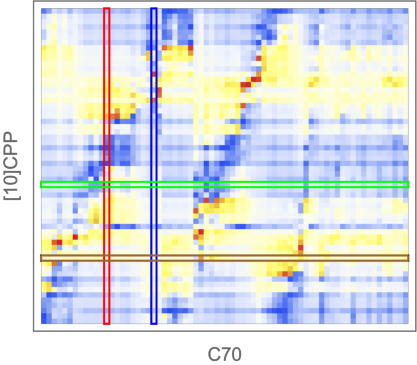
\includegraphics[width=\linewidth/2]{media/cpp-10-c70-xx.pdf}};
\node[below right, anchor=base] at (\linewidth/2,0) {{\bfseries b}};
\node[below right] at (\linewidth/2,.5) {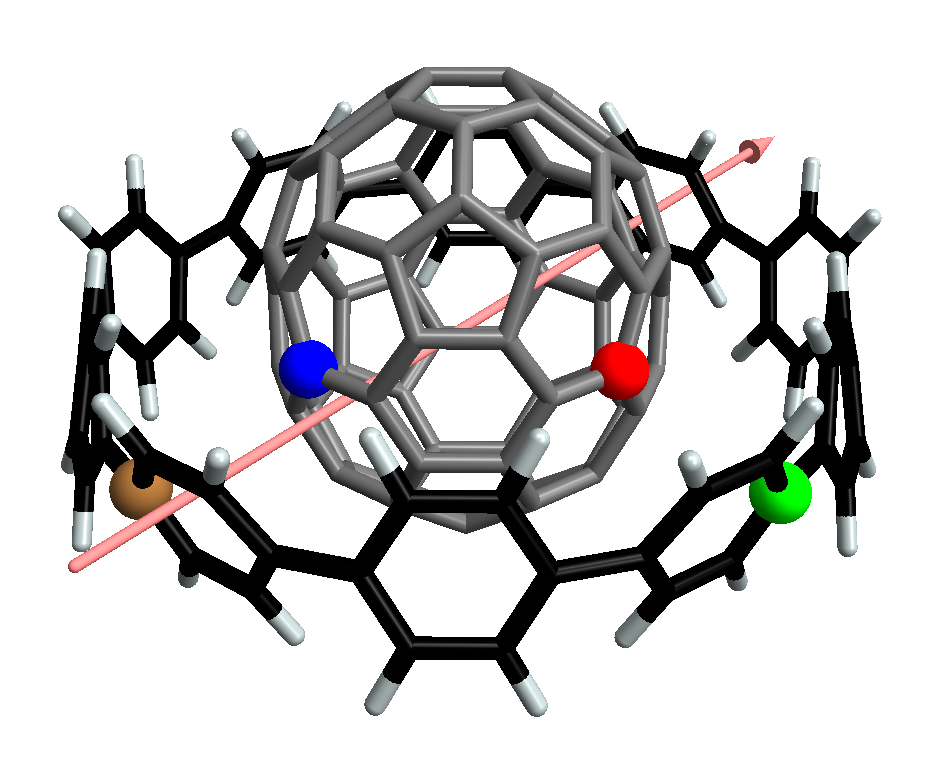
\includegraphics[width=\linewidth/2]{media/cpp-10-c70-marked-atoms-xx.pdf}};
\end{tikzpicture}
}
\caption{\textbf{Intermolecular part of the static nonlocal polarizability in [10]CPP--C$_{70}$.}
The heat map (\textbf a) shows the carbon--carbon $xx$ elements of the polarizability, with yellow/red and blue colors corresponding to the positive and negative values.
The colored stripes denote the atoms depicted with the corresponding color in the molecular structure (\textbf b).
The pink arrow shows the $x$ axis.
}\label{fig:pol-off}
\end{figure}

The off-diagonal blocks, $\boldsymbol\alpha_\text{hg}$, in the nonlocal polarizability encode the majority of the intermolecular many-body effects, and are directly related to the binding energy,
\begin{equation}
  E_\text{int,MBD}=\frac1{4\pi}\int_0^\infty\mathrm du\operatorname{Tr}_{p,\mathbb R^3}\big(\boldsymbol\alpha_\text{hg}(\mathrm iu)\mathbf T_\text{hg}\big)+O(\mathbf T_\text{hg}^3)
\end{equation}
(This expression is second-order in the intermolecular coupling, but infinite-order in the intramolecular coupling, so it contains, for instance, all three-atom Axilrod--Teller terms, which are second-order in intermolecular coupling and first-order in intramolecular coupling.)
Figure~\ref{fig:pol-off} shows the off-diagonal part of the polarizability in [10]CPP--C$_{70}$.
In the Hamiltonian formulation of the MBD method, the off-diagonal polarizability translates into the difference in the coupled oscillations between the full complex and the isolated host and guest, analyzed in the next section.

\section{Charge polarization due to $\uppi$--$\uppi$ interactions}

\begin{figure}
\makebox[\textwidth][c]{
\begin{tikzpicture}
\node[below right, anchor=base] at (0,0) {{\bfseries a}};
\node[below right] at (-.5,.5) {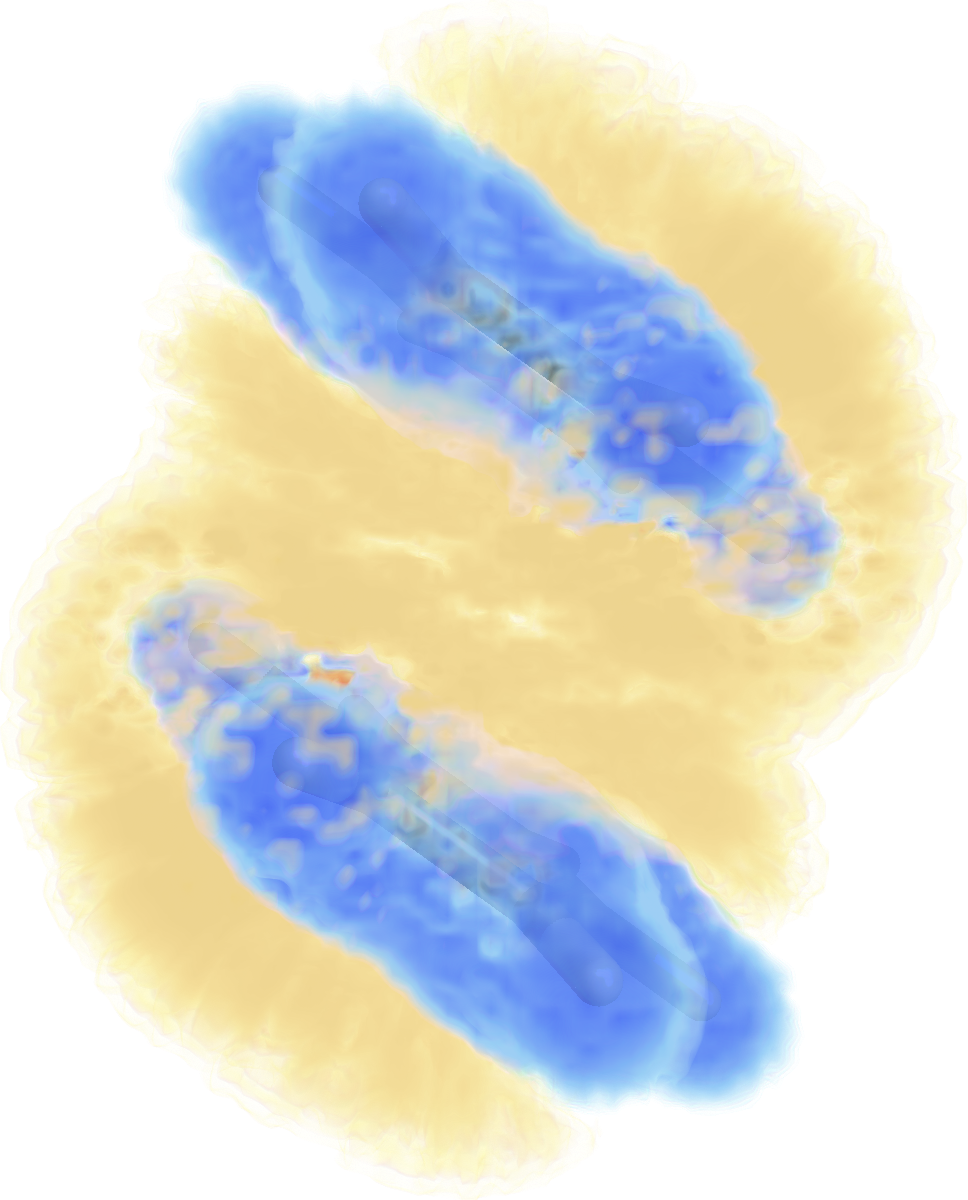
\includegraphics[width=2.1in]{media/dens-bz-dimer-ts.png}};
\node[below right, anchor=base] at (\linewidth/3+5,0) {{\bfseries b}};
\node[below right] at (\linewidth/3+6,.5) {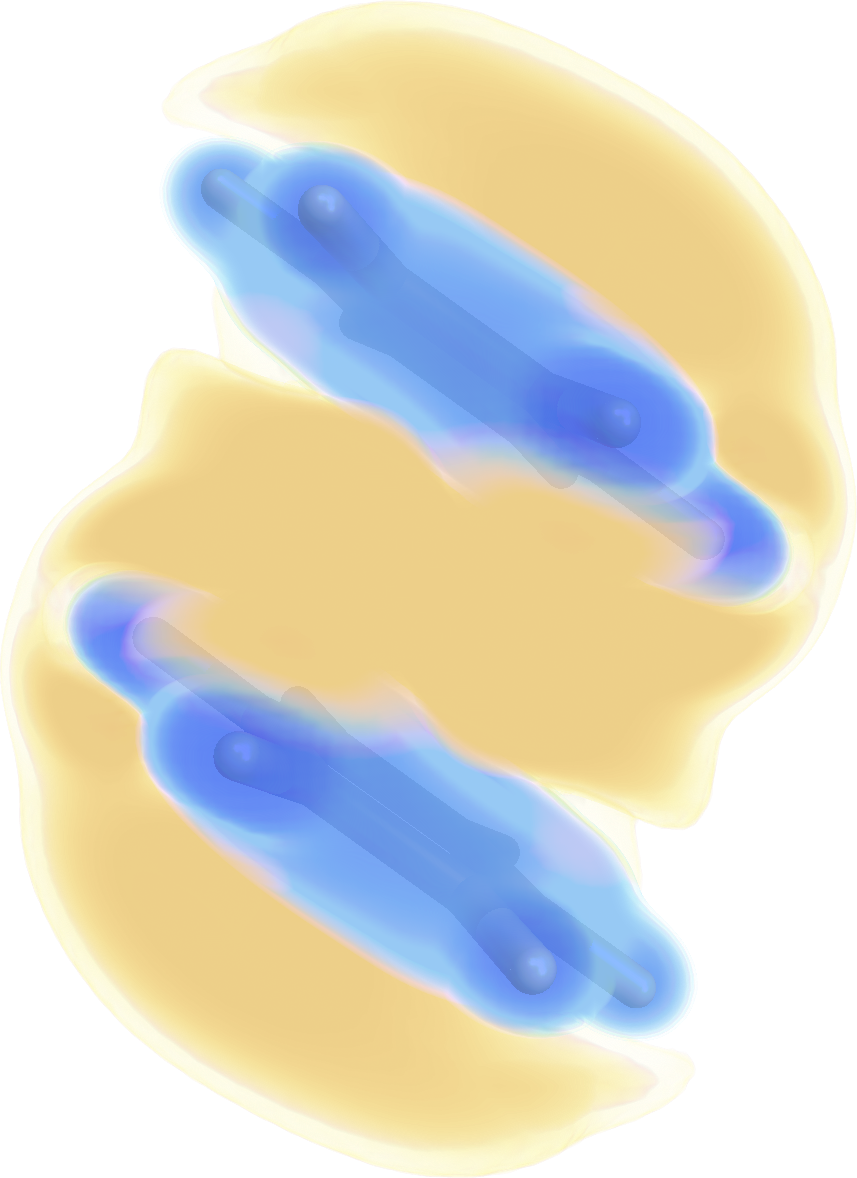
\includegraphics[width=2in]{media/dens-bz-dimer.png}};
\end{tikzpicture}
}
\caption{\textbf{Charge polarization due to vdW interactions.}
Electron density difference (charge polarization) induced by vdW interactions between the benzene dimer and isolated monomers calculated with the PBE+TS XC functional (\textbf a) and the MBD Hamiltonian (\textbf b).
Yellow and blue color represent accumulation and depletion of the charge density, respectively.
The magnitude of the polarization is mapped to color saturation, with 50\% corresponding to $2\times10^{-5}$ (a.u.).
}\label{fig:density-benzene}
\end{figure}

This section gives some evidence that the MBD Hamiltonian is capable of modeling more aspects of the full electronic system than just its long-range correlation energy.
VdW interactions usually induce only a small change in the electronic density~\cite{ThonhauserPRB07,VydrovJCP08}, but can also lead to substantial polarization with measurable effects~\cite{FerriPRL15}.
In the many-body perturbation picture, the long-range intermolecular Coulomb force induces virtual excitations to higher-energy one-particle states, which are always more diffused than the occupied states.
As a result, the electron density shifts to the outer regions of the atoms.
In DFT, the local KS potential becomes slightly slower decaying with increasing distance from the atoms, which again results in the electron density shifting somewhat outwards.
An example of this phenomenon in the case of benzene dimer is shown in Figure~\ref{fig:density-benzene}a, calculated with the PBE+TS XC functional~\cite{FerriPRL15}.
In MBD, the interaction between the molecules induces new collective nonlocal oscillations that have on average lower energies than in the isolated fragments, and since oscillators with lower ground-state energy have more diffused wave functions, this leads to a more diffuse total charge density of the oscillators calculated with~\eqref{eq:mbd-density}.
(This approach is different from doing DFT+MBD calculations self-consistently, where the total density would be of the real electrons, only slightly modified by $\delta E_\text{MBD}[n]/\delta n(\mathbf r)$.)
Comparison on the benzene dimer of the KS-DFT charge polarization due to vdW interactions and of the MBD oscillator polarization (Figure~\ref{fig:density-benzene}) shows a remarkable match between the two approaches.
This suggests that although the oscillators in the MBD Hamiltonian cannot in a reasonable way model the total electron density, they can model changes in the electron density induced by long-range electron correlation.
The agreement between the KS-DFT and MBD charge polarizations is even quantitative, with 0.0101 and 0.0097 displaced electrons (integral of $\max(0,\Delta n)$), respectively.

\begin{figure}
\makebox[\textwidth][c]{
\begin{tikzpicture}
\node[below right, anchor=base] at (0,0) {{\bfseries a}};
\node[below right] at (-.5,.5) {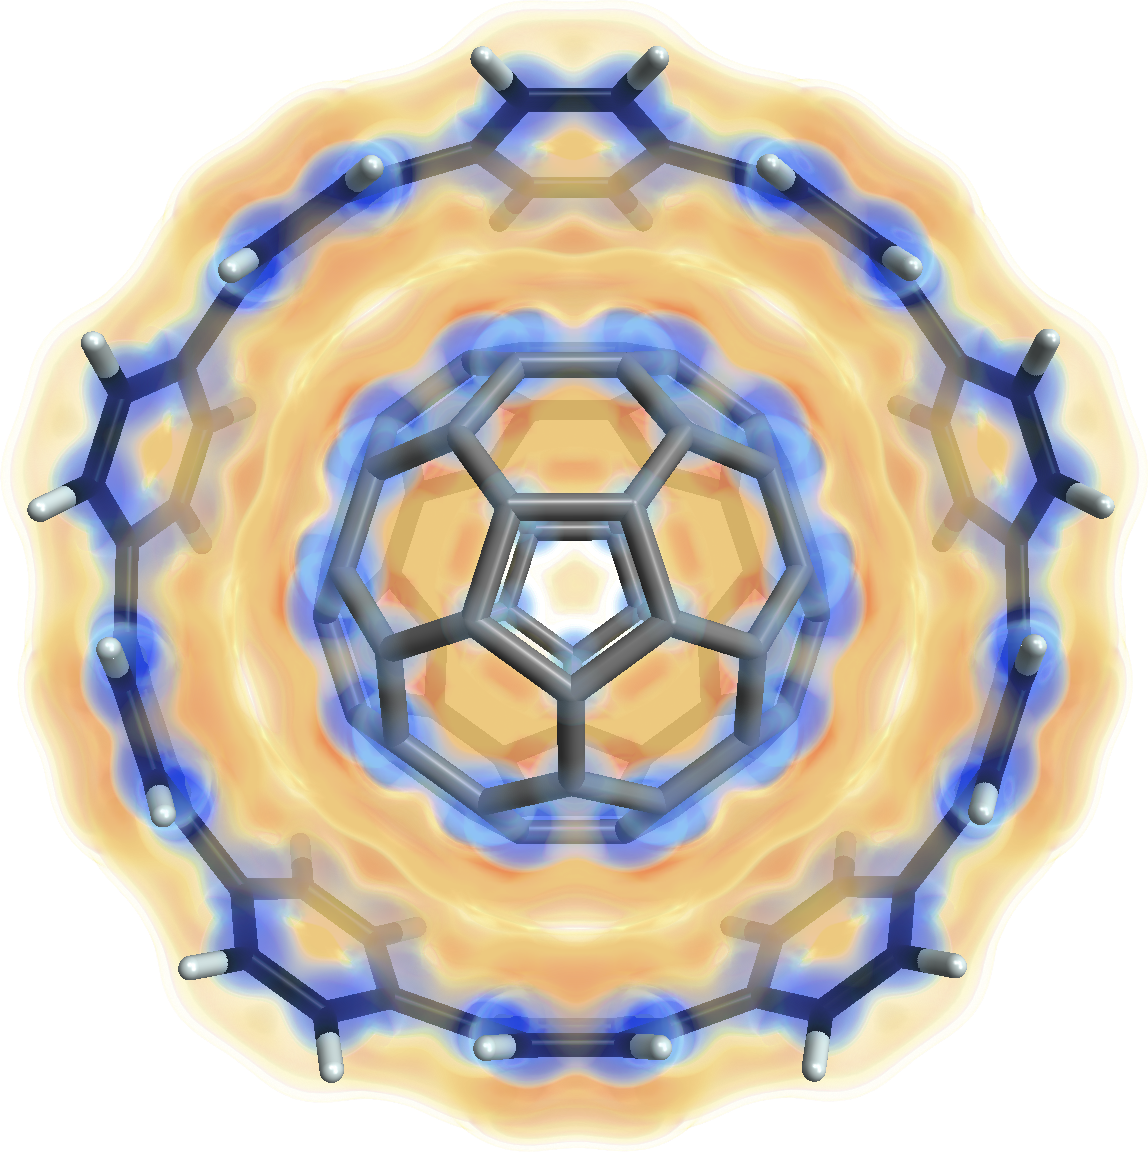
\includegraphics[width=\linewidth/3]{media/7-pol-density.png}};
\node[below right, anchor=base] at (\linewidth/3-5,0) {{\bfseries b}};
\node[below right] at (\linewidth/3-6,.5) {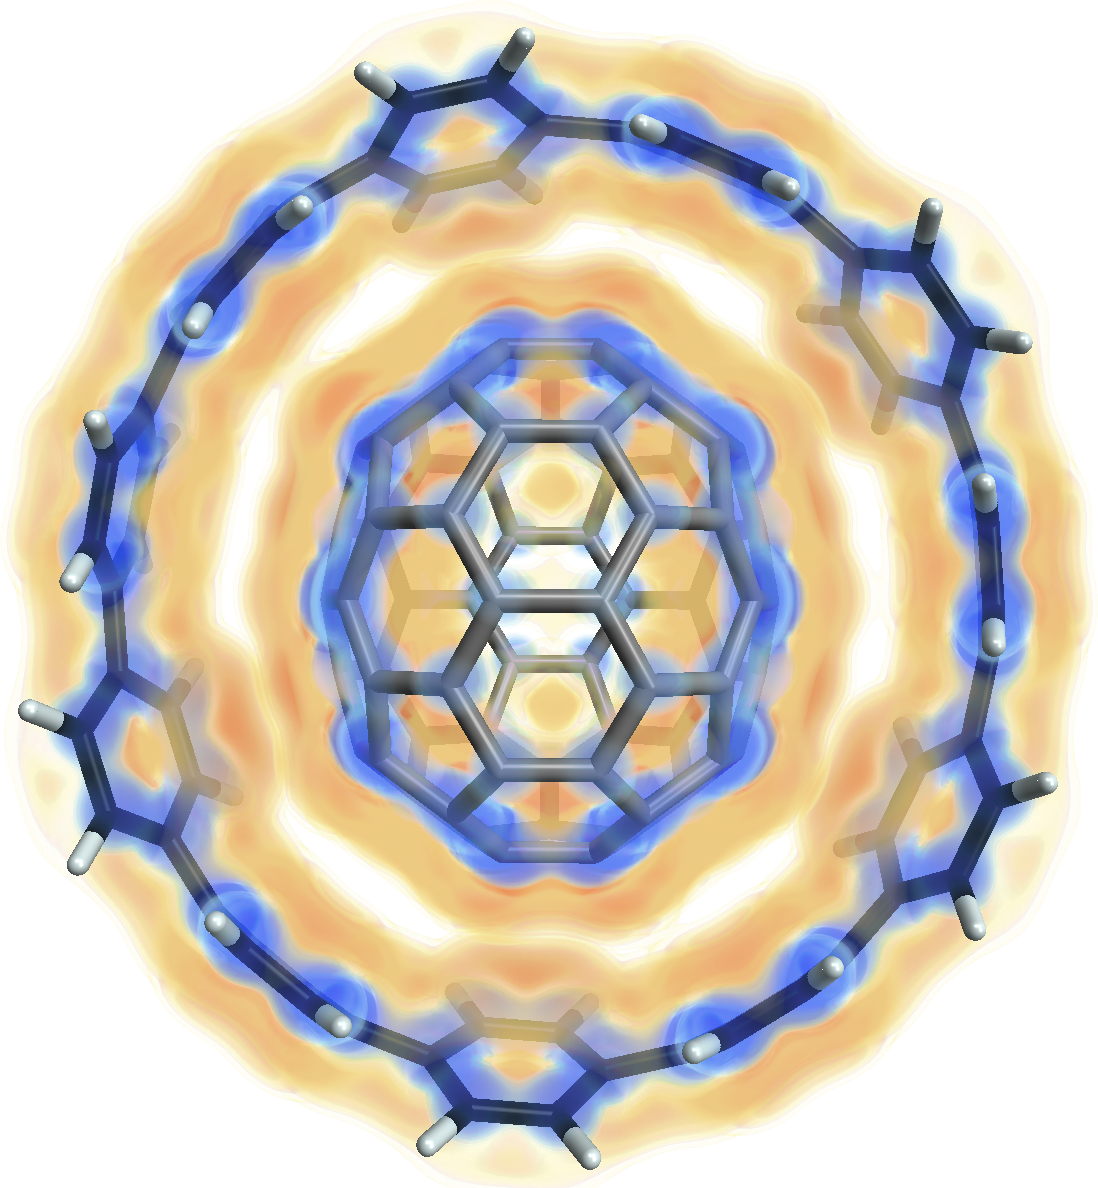
\includegraphics[width=\linewidth/3]{media/8-pol-density.png}};
\node[below right, anchor=base] at (2*\linewidth/3,0) {{\bfseries c}};
\node[below right] at (2*\linewidth/3-.5,.5) {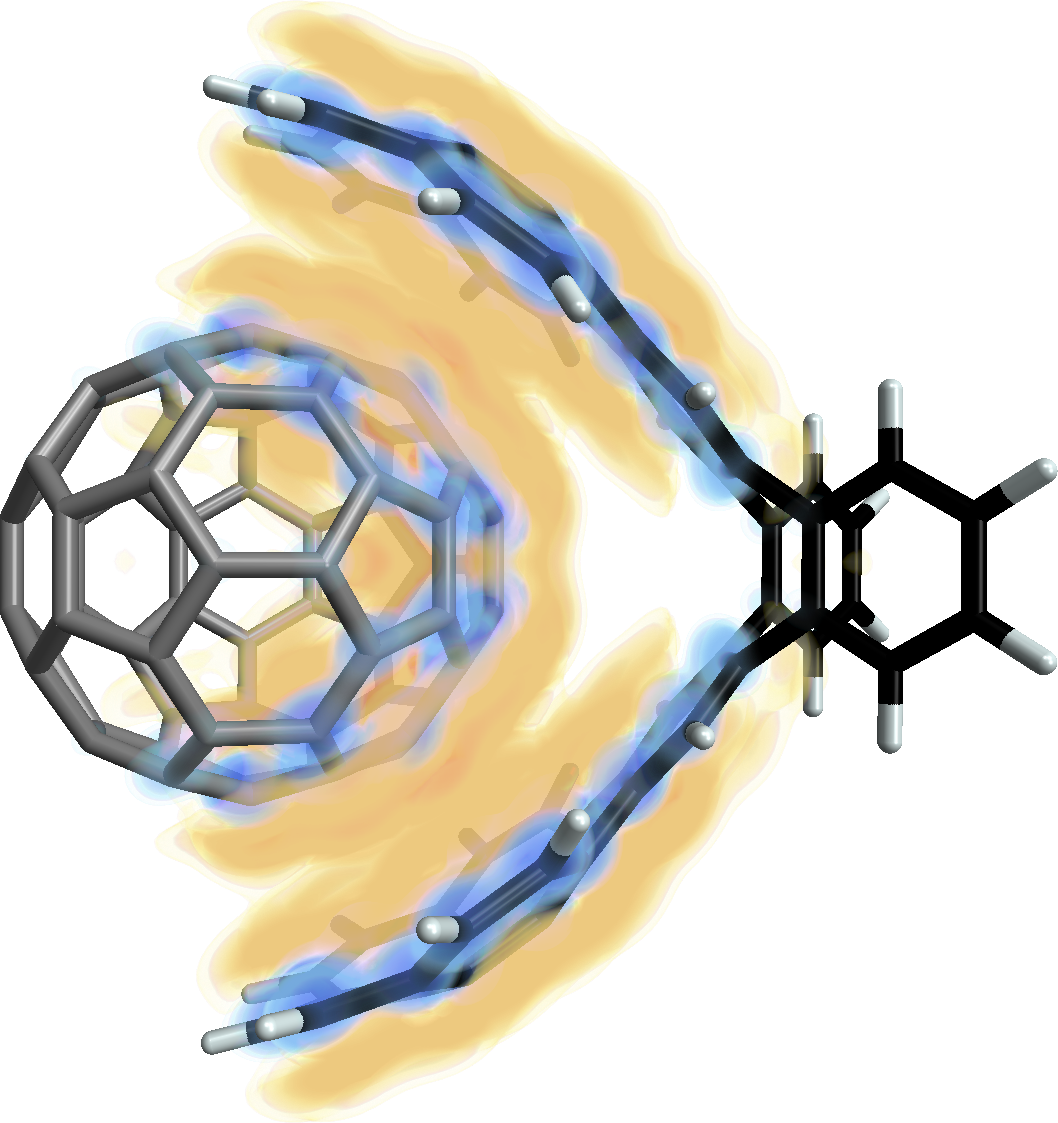
\includegraphics[width=\linewidth/3]{media/4b-pol-density.png}};
\end{tikzpicture}
}
\caption{\textbf{Charge polarization due to vdW interactions.}
The same visualization as in Figure~\ref{fig:density-benzene} for the three supramolecular complexes in Figure~\ref{fig:pipi-structures}.
}\label{fig:density-supra}
\end{figure}

Turning back to the supramolecular complexes, their charge polarization due to vdW interactions as calculated from the MBD density is shown in~\ref{fig:density-supra}.
The charge polarization gives an indirect measure of which spatial parts of the monomers contribute most to the binding.
Comparison of the complexes indicates that the charge fluctuations on the fragments are relatively well separated in the [11]CPP complex, but not in the [10]CPP complex, resulting in stronger many-body effects beyond the second-order (pairwise) expansion of the long-range correlation energy in [10]CPP--C$_{70}$.
This explains the stronger overbinding of the [10]CPP complex by the D3 method.

\section{VdW interactions as collective oscillations}

\begin{figure}
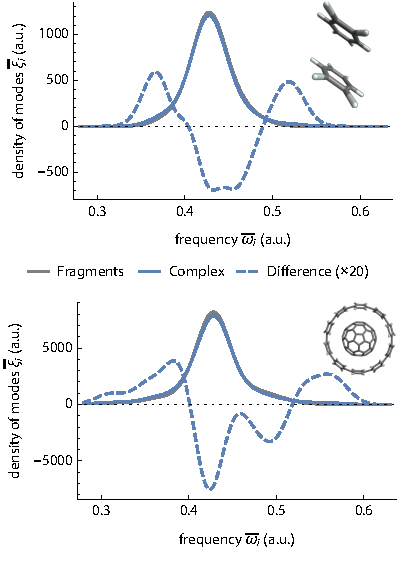
\includegraphics[width=3.5in]{media/doses.pdf}
\caption{\textbf{MBD densities of states.}
Distributions of the coupled-oscillator energies smoothed with Gaussian broadening of 0.06\,eV.
}\label{fig:mbd-dos}
\end{figure}

The polarization of the MBD charge densities due to intermolecular interactions is a combined effect of all the coupled oscillation modes.
This section analyzes the individual modes and their relation to the total binding energy.
Solving the MBD Hamiltonian for the complex and the isolated fragments leads to different modes with different energies.
Figure~\ref{fig:mbd-dos} shows that the distribution of the energies is broadened in the complex with respect to the fragments, so the binding mechanism is not a simple general shift of all the energies.
Rather, to first order in $\mathbf T_\text{hg}$, the energy spectrum is symmetrically broadened, with no change to the total energy, and only in second order in $\mathbf T_\text{hg}$ is the whole spectrum shifted to lower energies, leading to binding.
This is in contrast to orbital hybridization in molecules, where the energy splitting can be considered symmetric and the covalent binding arises from partial occupancy.
In the MBD ground state, none of the coupled modes are occupied, the total energy is the energy of the zero-point fluctuations, and the binding arises from an asymmetric split of the subsystem energy levels.

\begin{figure}
\makebox[\textwidth][c]{
\begin{tikzpicture}
\node[below right, anchor=base] at (0,0) {{\bfseries a}};
\node[below right] at (-.5,.5) {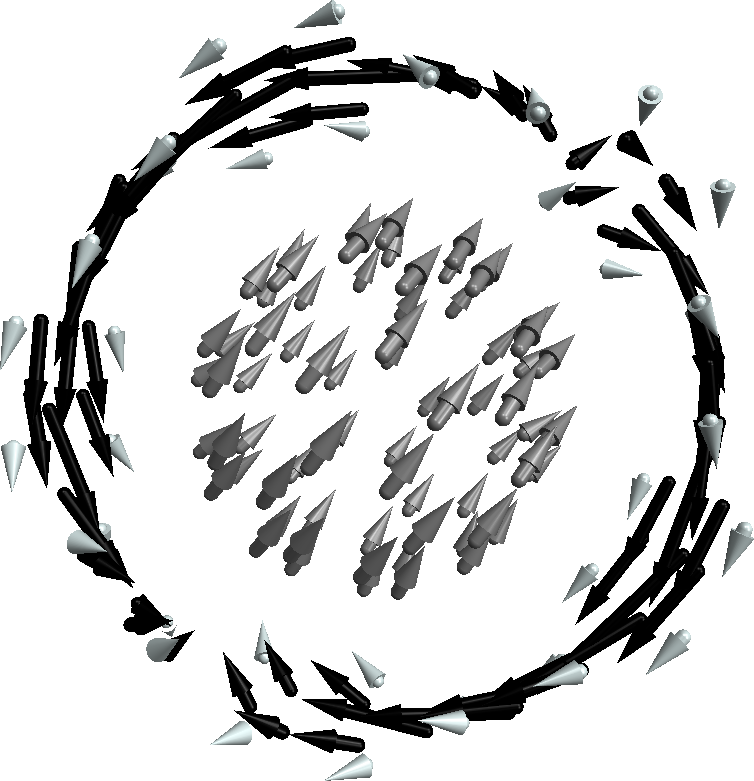
\includegraphics[width=\linewidth/3]{media/7-mode-2.png}};
\node[below right, anchor=base] at (\linewidth/3-5,0) {{\bfseries b}};
\node[below right] at (\linewidth/3-6,.5) {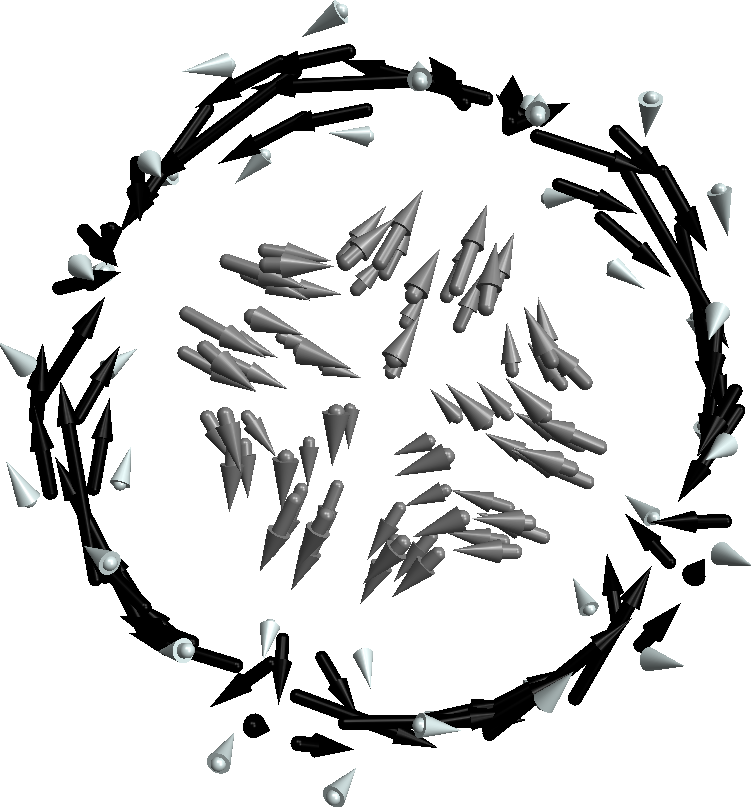
\includegraphics[width=\linewidth/3]{media/7-mode-7.png}};
\node[below right, anchor=base] at (2*\linewidth/3,0) {{\bfseries c}};
\node[below right] at (2*\linewidth/3-.5,.5) {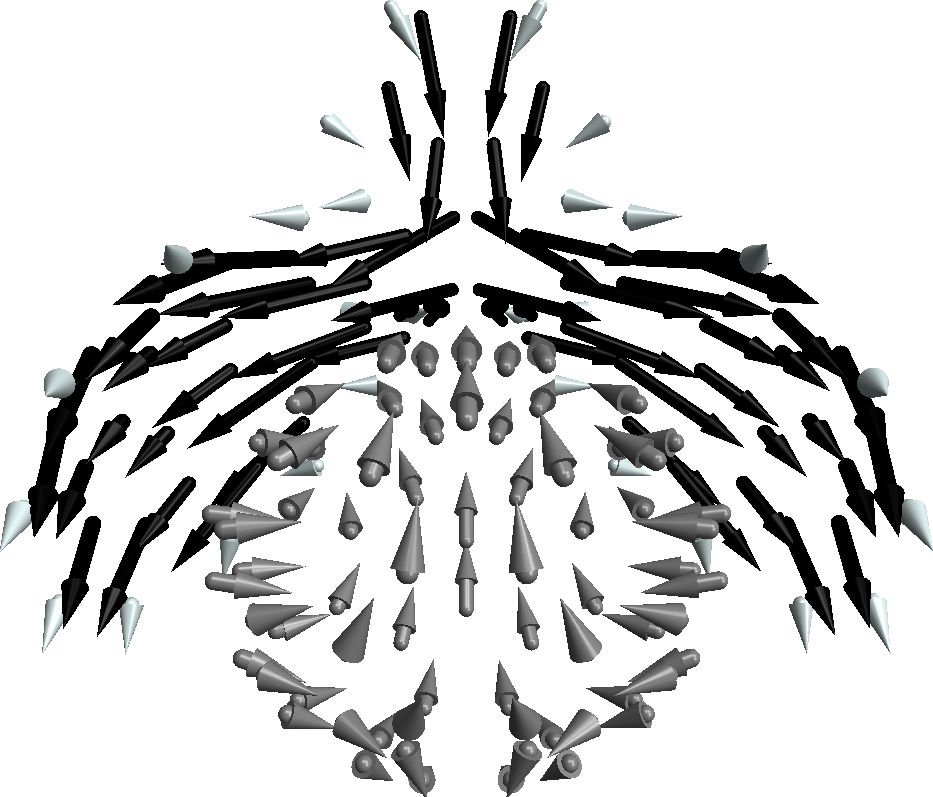
\includegraphics[width=\linewidth/3]{media/4b-mode-7.png}};
\end{tikzpicture}
}
\caption{\textbf{Most binding oscillation modes.}
The doubly degenerate most binding (\textbf a) and second most binding (\textbf b) oscillation mode of [10]CPP--C$_{70}$, and the most binding mode of buckycatcher--C$_{70}$.
The arrow on each atom denotes an in-phase dipole oscillation.
}\label{fig:mbd-modes}
\end{figure}

Using the decomposition technique from Section~\ref{sec:decom}, we can identify oscillation modes that contribute most to the binding energy.
The decomposition in~\eqref{eq:decom-1} in terms of the coupled modes of the whole complex turns out not to be very useful, because the most organized and collective modes contribute both positively and negatively.
In contrast, decomposing the binding energy along the coupled modes of the individual subsystems as in~\eqref{eq:decom-2} leads to mostly binding contributions.
To transform back to the full system, we multiply this decomposition by $\mathbf P^{\circ2}$.
The most contributing coupled modes (Figure~\ref{fig:mbd-modes}) have clear interpretation as global dipole and quadrupole oscillations.
These results suggest that an alternative to the pairwise picture of vdW interactions as correlation between dipoles and quadrupoles on pairs of atoms is a collective picture where the whole electronic system oscillates in a wave-like fashion.
These molecular oscillations, also called molecular plasmons in other contexts~\cite{LauchnerNL15}, are of the same nature as plasmons in metals or electronic dipole waves in nanomaterials~\cite{AmbrosettiS16}.

\begin{figure}
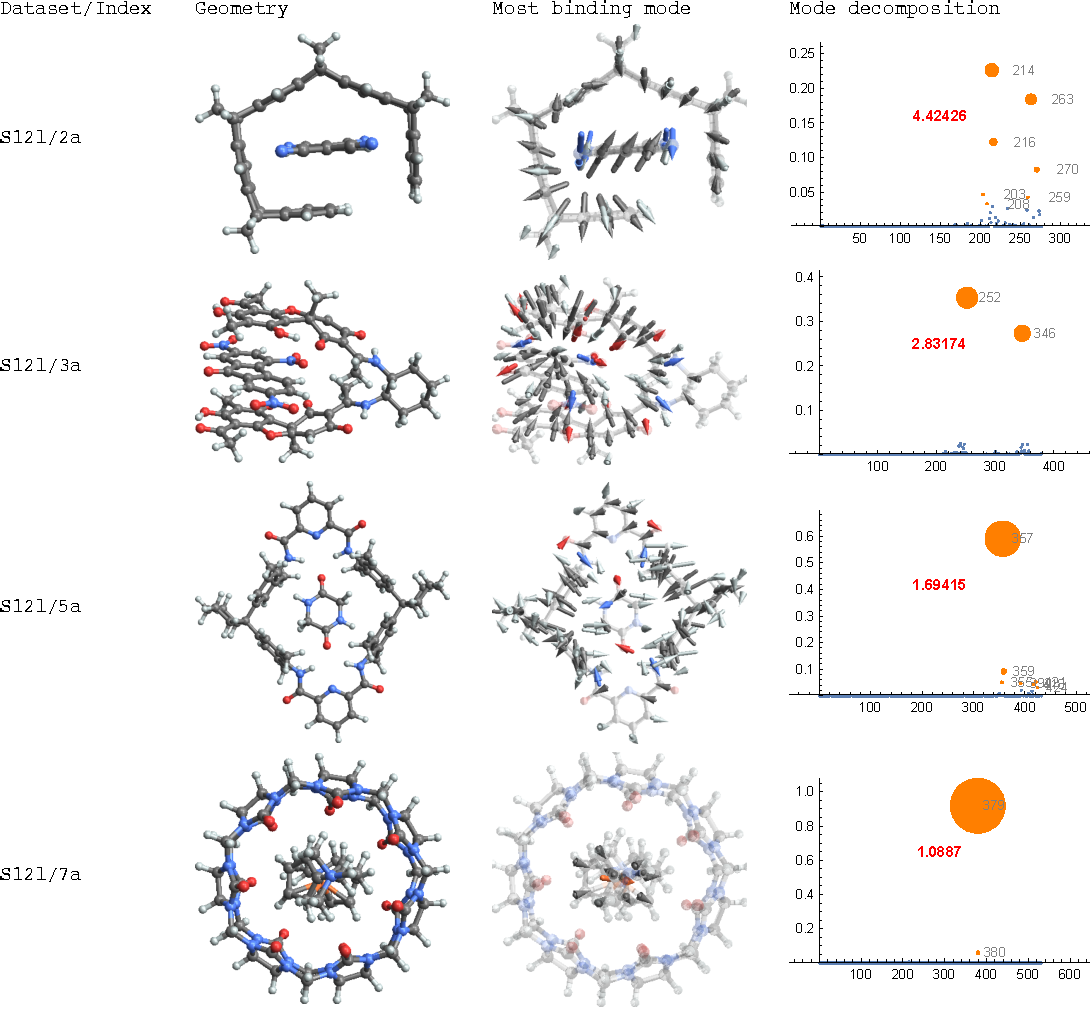
\includegraphics[width=\linewidth]{media/modes-decom-1.pdf}
\caption{\textbf{Most binding oscillation modes in different types of binding.}
Each row in the table corresponds to a complex from the S12L benchmark dataset \citep{RisthausJCTC13}.
The right-most column shows squares of the coefficients of the decomposition of the most binding mode of the complex into the modes of the monomers.
The number in red is the inverse of the largest coefficients.
The oscillation arrows are put only on atoms where the magnitude of the dipole is larger than 10\% of the maximum magnitude.
}\label{fig:mbd-decom-s12l}
\end{figure}

So far, we showed that the binding in supramolecular $\uppi$--$\uppi$ complexes can be understood in terms of collective wave-like electronic fluctuations.
Next, we demonstrate that this is quite characteristic of these systems, and the oscillations in other types of complexes are either localized or disorganized.
Figure~\ref{fig:mbd-decom-s12l} shows the most binding oscillation modes of two $\uppi$--$\uppi$ complexes (2a and 3a) and two complexes which are bound by unspecific vdW and electrostatic interactions (5a and 7a).
As in the three fullerene complexes, the most binding mode in the $\uppi$--$\uppi$ complexes is uniformly delocalized over the whole complex.
Furthermore, the decomposition of these modes into the subsystem modes shows that they are not dominated by a single subsystem mode, but are a combination of several subsystem modes, indicating their strong coupling.
In contrast, the most binding modes of the non-$\uppi$--$\uppi$ complexes are rather disorganized, and even if delocalized, the motion has no collective nature.
Accordingly, these modes are dominated by a single subsystem mode, so instead of strong coupling as in the stacked complexes, here a single subsystem mode induces only weak oscillations on the other subsystem.
This suggests that the long-range electronic oscillations in these systems could be effectively decomposed into pairwise contributions, and indeed, the pairwise approaches are much more accurate for these types of complexes than for the $\uppi$--$\uppi$ complexes.

\section{Testing nonequilibrium geometries}

\begin{sidewaysfigure}
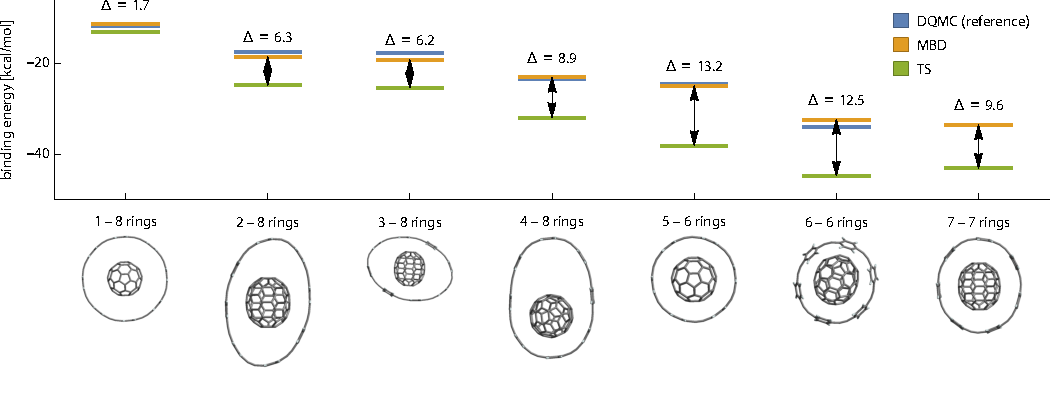
\includegraphics[width=\linewidth]{media/cppa-complexes.pdf}
\caption{\textbf{Binding energies of $C_{70}$ in [$N$]-cycloparaphenyleneacetylene.}
$N$ is the number of rings in the host CPPA molecule.
All structures are local minima of the potential energy surface, but not necessarily global minima.
Both the MBD and TS methods were combined with the PBE functional.
The $\Delta$ values are the difference between PBE+MBD and PBE+TS in kcal/mol.
}\label{fig:mbd-noneq}
\end{sidewaysfigure}

All structures investigated in the previous sections were equilibrium structures.
This section presents an extension of the DQMC benchmark of the MBD model to nonequilibrium structures.
The higher-order many-body effects are sensitive to the symmetry of the system, and it is imaginable that some hidden error-canceling mechanism in equilibrium structures could lead to the high accuracy of MBD for the three C$_{70}$ complexes.
However, Figure~\ref{fig:mbd-noneq} shows that the excellent agreement between PBE+MBD and DQMC is achieved even for several nonequilibrium geometries, with the largest deviation of 1.7\,kcal/mol (5\%).
In contrast, the pairwise PBE+TS method overbinds the complexes by 2 to 13 kcal/mol.
The nonuniform difference between TS and MBD shows that higher-order many-body effects are more sensitive to the geometry than the baseline pairwise vdW energy.
In general, the relative difference between TS and MBD is larger in more tightly stacked geometries, which is in line with the larger error of D3 on the [10]CPP--C$_{70}$ complex.
